
\documentclass[12pt]{article}

\usepackage{graphics}
\usepackage{epsfig}

\setlength{\textwidth}{17cm}
\setlength{\textheight}{25cm}
\setlength{\topmargin}{-1cm}
\setlength{\leftmargin}{-1cm}


\newcommand{\bea}{\begin{eqnarray}} 
\newcommand{\eea}{\end{eqnarray}} 

\newcommand{\aww}{A_{\scriptstyle WW}}
\newcommand{\alphah}{\mbox{$\hat{\alpha}$}}

%%%%%%%%%%%%%%%%%%%%%%%%%%%%%%%%%%%%%%%%%%%%%%%%%%%%%%%%%%%%%%%%%%%%%%%%%%%
\begin{document}
\section{introduzione}
bla bla
in cui parlate dell'articolo \cite{paper1} in cui viene contestata la tesi
esposta in \cite{paper2}

\clearpage
\section{primo capitolo}
\label{mathsimbol}
ciao ciao 

i simboli matematici vanno inclusi tra dollari \\
$x^y$ ma attenzione $x^2y$ d\`a un risultato diverso da $x^{2y}$\\
le parentesi tonde e quadre si scrivono normalmente\\
le parentesi graffe con il $\backslash$ \{ e \}\\
le frazioni sono $\frac{a+b}{c+d}$\\
la radice quadrata $\sqrt{1-x^2}$\\
le parentesi si possono adattare alla dimensione del loro argomento
a patto di scrivere\\
$\left[ \frac{a+b}{c+d} \right]$ 
diverso da
$[ \frac{a+b}{c+d} ]$ \\
sono simboli matematici (ovvero che vanno tra dollari) le lettere greche\\
$\alpha\beta\gamma\delta\epsilon\cdots\Gamma\Delta\Phi\Psi\Omega\cdots$\\
e una raccolta di svariati simboli come\\
$\pm\,\mp\,\times\,\bullet\,\wedge\,\leq\,\geq\,\gg\,\ll\,\sim\,\simeq
\,\equiv\,\perp\,\propto$\\
e varie frecce\\
$\to\,\leftarrow\,\rightarrow\,\Leftarrow\,\Rightarrow$\\
all'interno del modo matematico, le scrittte testuali appaiono in corsivo
$come per esempio$ \\
per scrivere le funzioni elementari si usa di nuovo il $\backslash$
$\sin\,\cos\,\ln\cdots$\\
per centrare un'espressione matematica si usa il doppio dollaro
$$
x_{1,2} = \frac{-b\pm\sqrt{b^2-4\,a\,c}}{2a}
$$
per scrivere una equazione che venga numerata si usa
\begin{equation}
z=a\, x + b\, y
\end{equation}
per scrivere un sistema di equazioni si usa
\begin{eqnarray}
a &=& a_1 y + a_2 z \\
b &=& \sqrt{x^2+y^2}\label{secondaeq}
\end{eqnarray}
per evitare l'apparire della numerazione di ciascuna equazione
\bea
a &=& a_1 y + a_2 z \nonumber\\
b &=& \sqrt{x^2+y^2}\nonumber
\eea
per mettere parentesi "grandi"\\
$$
\left\{
\begin{array}{c}
a\\
b\\
x+y
\end{array}
\right.
$$

\clearpage

\subsection{alcuni dettagli}
proviamo a specificare qualcosa \alphah\\
per esempio possiamo riferirci alla figura \ref{cspph} senza dover 
introdurre a mano un numero\\
la stessa cosa vale per le equazioni numerate come p.es. la eq.\ref{secondaeq}

\section{immagini}
\begin{figure}
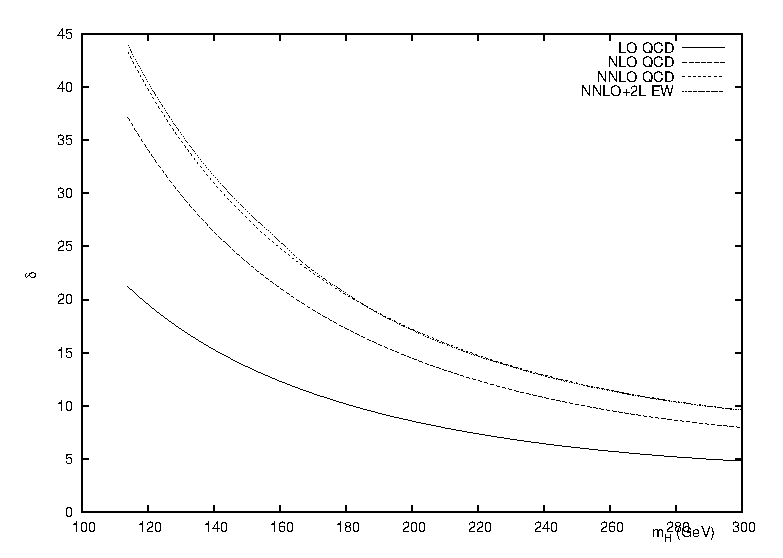
\includegraphics[height=100mm,angle=0]{pph.ps}
\caption{sezione d'urto adronica per la produzione di Higgs a LHC}
\label{cspph}
\end{figure}




\clearpage
\section{ringraziamenti}
ringraziamo lo staff di LCM per il supporto offerto alla nostra attivit\`a
\appendix{appendice A}
alcuni dettagli
\appendix{appendice B}
e altri ancora

\begin{thebibliography}{99}
\bibitem{paper1} primo articolo che citate

\bibitem{paper2} secondo articolo che citate

\end{thebibliography}

\end{document}
